% Based on Jeremy Siek's DLS slides
\documentclass[12pt]{beamer}
%\usecolortheme{seagull}
%\usecolortheme{wolverine} yuk
%\usecolortheme{beetle}
\usecolortheme{dove} % black on white
\usepackage[T1]{fontenc}
\usepackage{garamond}
\usefonttheme{serif}
\usepackage{multicol}
\usepackage{pifont}
\usepackage{etex}
\usepackage{graphicx}
\usepackage{amsmath}
\usepackage{amsthm}
\usepackage{amssymb}
\usepackage{semantic}
\usepackage[all]{xy}
\usepackage{color}
\usepackage{listings}
\usepackage{fancybox}
\usepackage{stmaryrd}
\usepackage{rotating}
\usepackage{wasysym}
\usepackage{ulem}

\usepackage{enumitem}
\setitemize{label=\usebeamerfont*{itemize item}%
  \usebeamercolor[fg]{itemize item}
  \usebeamertemplate{itemize item}}
  \setlist{itemsep=1ex}



\newcommand{\Gbox}[1]{\colorbox{lightgray}{#1}}
\newcommand{\Rbox}[1]{\colorbox{pink}{#1}}

\newcommand{\featstart}{\hfill}
\newcommand{\featend}{\hfill\hfill}
\newcommand{\feat}[1]{{\featstart#1\featend}}

\newcommand{\Topcircle}{\begin{turn}{270}\Leftcircle\end{turn}}
\newcommand{\BOTTOMCIRCLE}{\begin{turn}{270}\RIGHTCIRCLE\end{turn}}
\newcommand{\halfcircle}{\parbox{0in}{\Topcircle}\parbox{1.65ex}{\BOTTOMCIRCLE}{}}

\newcommand{\featY}{\feat{\CIRCLE}} % Has feature fully
\newcommand{\featP}{\feat{\halfcircle}} % Has feature partially
\newcommand{\featN}{\feat{\Circle}} % Does not have feature


\newcommand{\labeltag}[1]{\label{#1}\tag{\textsc{#1}}}
\newcommand{\type}{\vdash}
\newcommand{\typeS}{\vdash_{STLC}}
\newcommand{\typeG}{\vdash}
\newcommand{\typeCC}{\vdash_{C}}

\newcommand{\evall}{\Downarrow }
\newcommand{\evallS}{\Downarrow_{STLC} }
\newcommand{\evallG}{\Downarrow}
\newcommand{\evallCC}{\Downarrow_{C}}
\newcommand{\evallD}{\Downarrow_{DTLC}}

\newcommand{\reduce}{\longrightarrow}
\newcommand{\becomes}{\longrightarrow}

\newcommand{\EE}{{\cal E}}
\newcommand{\FF}{{\cal F}}
\newcommand{\Hole}{\Box}

\newcommand{\divergeG}{\Uparrow}
\newcommand{\subtype}{<:}
\newcommand{\consis}{\sim}

\newcommand{\embed}[1]{\lceil #1 \rceil}
\newcommand{\bl}[1]{{\color{blue} #1}}
\newcommand{\rd}[1]{{\color{red} #1}}
\newcommand{\gr}[1]{{\color{green} #1}}
\newcommand{\pr}[1]{{\color{purple} #1}}
\newcommand{\kw}[1]{\mathtt{#1}}

\newcommand{\labels}[1]{\mathit{labels}(#1)}
\newcommand{\static}[2]{\mathit{static}(#1,#2)}
\newcommand{\safe}[1]{\mathrel{\mathit{safe}} #1}
\newcommand{\lo}[1]{\overline{#1}}
\newcommand{\rng}[1]{\mathit{rng}(#1)}

\newcommand{\semi}{\mathbin{;}}
\newcommand{\id}{\key{id}}
\newcommand{\Id}[1]{\id_{#1}}
\newcommand{\fail}[3]{\bot^{#1}_{#2 \Rightarrow #3}}
\newcommand{\Fail}[1]{\bot^{#1}}
\newcommand{\FAIL}[3]{\bot^{#2}}
\newcommand{\qu}[2]{{{#2}\query^{#1}}}
\newcommand{\pl}[1]{{#1\pling}}
\newcommand{\query}{\mathtt{?}}
\newcommand{\pling}{\mathtt{!}}

\newcommand{\bcfun}[1]{\langle\!\langle #1 \rangle\!\rangle}
\newcommand{\MergeT}{\sqcap}
\newcommand{\RefC}[1]{\key{Ref}(#1)}
\newcommand{\error}{\key{error}}
\newcommand{\rtti}[2]{#1(#2)_{\mathsf{rtti}}}
\newcommand{\val}[2]{#1(#2)_{\mathsf{val}}}

\newcommand{\Obj}{\key{Obj}}
\newcommand{\String}{\key{String}}
\newcommand{\Double}{\key{Double}}

%\newcommand{\If}[3]{\key{if}\,#1\key{if}\,#2\key{if}#3}


\newcommand{\ba}{\begin{array}}
\newcommand{\ea}{\end{array}}
\newenvironment{stack}{\ba{@{}l@{}}}{\ea}
\newenvironment{branch}{\left\{\ba{@{}l@{\qquad}l@{}}}{\ea\right\}}
\newenvironment{syntax}{\[\ba{l@{\;\;}lcl}}{\ea\]}
\newcommand{\dotspace}{.\,}
\newcommand{\key}[1]{\ensuremath{\mathtt{#1}}}
\newcommand{\Base}{B}
\newcommand{\dyn}{\star}
\newcommand{\Dyn}{\ensuremath{\dyn}}
\newcommand{\Int}{\key{Int}}
\newcommand{\Float}{\key{float}}
\newcommand{\Bool}{\key{Bool}}
\newcommand{\Str}{\key{String}}
\newcommand{\Ref}{\key{Ref}\,}
\newcommand{\lam}[1]{\lambda #1 \dotspace}
\newcommand{\Lam}[1]{\Lambda #1 \dotspace}
\newcommand{\by}{\mapsto}
\newcommand{\app}{\;\,}
\newcommand{\tapp}{\;\,}
\newcommand{\of}{{:}}
\newcommand{\tu}{{\to}}
\newcommand{\To}{\Rightarrow}
\newcommand{\Let}{\key{let}\;}
\newcommand{\Letrec}{\key{let}\,\key{rec}\;}
\newcommand{\In}{\key{in}\;}
\newcommand{\If}{\key{if}\;}
\newcommand{\Then}{\;\key{then}\;}
\newcommand{\Else}{\;\key{else}\;}
\newcommand{\True}{\key{true}}
\newcommand{\False}{\key{false}}
\newcommand{\as}{\mathrel{\key{as}}}
\newcommand{\op}{\mathit{op}}
\newcommand{\dom}[1]{\mathit{dom}(#1)}
\newcommand{\cod}[1]{\mathit{cod}(#1)}
\newcommand{\blame}[1]{\key{blame}\,#1}
\newcommand{\pblame}[2]{\key{blame}\,#1@#2}
\newcommand{\ledyn}{\sqsubseteq}
\newcommand{\IS}{\mathrel{\mathtt{is}}}
\newcommand{\cast}[1]{\overset{#1}{\Rightarrow}}
%\newcommand{\mkcast}[1]{\langle\!\langle#1\rangle\!\rangle}
\newcommand{\mkcast}[1]{(#1)}
\newcommand{\alloc}{\key{ref}\,}
\newcommand{\deref}{\texttt{!}}
\newcommand{\update}{\mathrel{\texttt{:=}}}
\newcommand{\all}[1]{\forall #1.\,}
\newcommand{\ftv}[1]{\mathrm{ftv}(#1)}
\newcommand{\CAST}[1]{\langle #1 \rangle}
\newcommand{\new}[1]{\nu #1.\;}
\newcommand{\case}[3]{\key{case}\,#1\,\key{of}\,\key{inl}\,x\Rightarrow\,#2\,| \,\key{inr}\,x\Rightarrow \,#3}
\newcommand{\join}[2]{#1 \sqcup #2 }
\newcommand{\meet}[2]{#1 \sqcap #2 }

\newcommand{\hy}[3]{#1 \overset{#2}{\curvearrowright} #3}

\newcommand*\oldmacro{}%
\let\oldmacro\insertshorttitle%
\renewcommand*\insertshorttitle{%
  \oldmacro\hfill%
  \insertframenumber\,/\,\inserttotalframenumber}

\setbeamertemplate{navigation symbols}{}
\setbeamertemplate{footline}[frame number]

%\newtheorem{definition}{Definition}
\newtheorem{conjecture}[theorem]{\translate{Conjecture}}
\newtheorem{proposition}[theorem]{\translate{Proposition}}

\lstdefinestyle{basic}{
%showstringspaces=false,
language=Python,
columns=fullflexible,
%basicstyle=\sffamily\small,%
basicstyle=\ttfamily,%
%columns=fixed,
%basewidth=0.49em,
%lineskip=0pt,
%escapechar=@,xleftmargin=1pc,%
keywordstyle=\ttfamily,
mathescape=true,%
moredelim=**[is][\color{blue}]{@}{@},
moredelim=[is][\color{red}]{|}{|},
moredelim=[is][\color{blue}]{~}{~},
%commentstyle=\rmfamily,%
%morekeywords={return,fix,var,proc,fun,func},%
%deletekeywords={int,bool}
}
\lstset{style=basic}

\newcommand{\lstsetgrift}{
  \lstset{%
    language=Lisp,
    basicstyle=\ttfamily\small,
    keywordstyle=\ttfamily\bfseries\small,
    columns=flexible,
    aboveskip=\smallskipamount,
    belowskip=\smallskipamount,
    xleftmargin=2pt,
    escapeinside={/+}{+/},
    mathescape=true,
    morekeywords=[1]{define,lambda,if,begin,letrec,let,let*,values,:,repeat,then,else,return,and,time,box,ref,unbox,box,ann},
    literate=
    {+}{{\textsf{+}}}1
    {-}{{\textsf{-}}}1
    {=>}{{$\rightarrow\;$}}2
    {lambda}{{$\boldsymbol{\lambda}$}}1
  }
}%%

\garamond

\title[Sound Gradual Typing]{Toward Efficient Sound Gradual Typing}
\author{Deyaaeldeen Almahallawi}
\institute[IU]{ Indiana University Bloomington}
\date[\today]{\today \\ \vspace{1cm} Joint work with Andre Kuhlenschmidt and Jeremy Siek}
%% \institute{\normalsize 
%%  Indiana University, Bloomington
%% }

% 3 hours

%\newcommand\footnotemark{}
%\renewcommand\footnoterule{}
\setbeamercolor{footnote mark}{fg=white}

\begin{document}

%===============================================================================
\frame{
\titlepage
}
%===============================================================================
\frame{
\frametitle{Gradual Typing}

\hspace{0.3in}
\begin{minipage}{0.7\textwidth}
{\Large Static}

\includegraphics[width=0.7\textwidth]{yinyang}
{\Large Dynamic}
\end{minipage}

}
%===============================================================================
\frame{
\frametitle{Efficient gradual typing}

\begin{itemize}
\item Challenges to Efficiency
\item Challenges to Evaluation
\item Space-efficient Coercions
\item Monotonic Coercions
\item Performance Comparison
\end{itemize}

}
%===============================================================================
\frame{
\frametitle{There is tension in the design space}

\[
\xymatrix{
    Efficient \ar@{<->}[rr]\ar@{<->}[dr] & & Sound \ar@{<->}[dl] \\
    & Interoperable & 
}
\]

\vspace{20pt}

\hspace{20pt}
\begin{tabular}{l|ccc}
Approach       & Sound & Efficient & Interoperable \\ \hline
erase types    & \featP & \featP & \featY \\
insert casts   & \featY & \featP & \featY \\
limit interop. & \featY & \featY & \featP
\end{tabular}

}
%===============================================================================
\frame{
\frametitle{Approach: insert casts}

\vspace{5pt}

Compile the GTLC to STLC + casts.

\vspace{5pt}

A cast has the form
\[
e' : T_1 \cast{} T_2
\]

\fbox{$\Gamma \vdash e \leadsto e' : T$}
\begin{gather*}
\inference
    {\Gamma \vdash e_1 \leadsto e'_1 : T \tu T' &
      \Gamma \vdash e_2 \leadsto e'_2 : T_2 \\
      T_2 \consis T}
    {\Gamma \vdash e_1 \app e_2 \leadsto e'_1 \app \rd{\mkcast{e'_2 : T_2 \cast{} T}} : T'}
\\[2ex]
\inference{\Gamma \vdash e_1 \leadsto e'_1 : \dyn & 
  \Gamma \vdash e_2 \leadsto e'_2 : T_2}
          {\Gamma \vdash e_1 \app e_2 \leadsto 
            \rd{\mkcast{e_1 : \dyn \cast{} \dyn \tu \dyn}}
            \app \rd{\mkcast{e_2 : T_2 \cast{} \dyn}} : \dyn}
\end{gather*}
%% where
%% \[
%% \mkcast{e' : T_1 \cast{} T_2} =
%% \begin{cases}
%%   e' & \text{if } T_1 = T_2 \\
%%   e' : T_1 \cast{} T_2 & \text{otherwise}
%% \end{cases}
%% \]

}
%===============================================================================
\frame{
\frametitle{Operational semantics of casts} % UD

\vspace{2pt}
\[
\begin{array}{llcl}
\text{Base types} & B &::=& \Int \mid \Bool\\
\text{Injection types} & I & ::= & B \mid \dyn \to \dyn \\
\text{Values} & v &::= &n \mid b \mid \lam{x\of T} e \mid \\
        &&& v : I \cast{} \dyn \mid v : T \tu T \cast{} T \tu T
\end{array}
\]
\begin{align*}
(v : I \cast{} \dyn) : \dyn \cast{} I & \reduce v \\
(v : I \cast{} \dyn) : \dyn \cast{} I' & \reduce \blame{} \quad
     \text{if } I \neq I'\\
v : B \cast{} B & \reduce v \\
v : \dyn \cast{} \dyn & \reduce v \\
(v : T_1 \tu T_2 \cast{} T'_1 \tu T'_2)\app v' & \reduce
  v \app (v' : T'_1 \cast{} T_1) : T_2 \cast{} T'_2 \\
v : T \cast{} \dyn & \reduce (v : T \cast{} I) : I \cast{} \dyn  \; ^\dagger \\
v : \dyn \cast{} T & \reduce (v : \dyn \cast{} I) : I \cast{} T \; ^\dagger 
\end{align*}

$\dagger \; \text{if } T \consis I, T \neq I, \text{ and } T \neq \dyn$
}
%===============================================================================
\frame{
\frametitle{Example}

\[
\begin{stack}
\begin{stack}
  (\kw{let}\ ((f\ (\lam{(y : \kw{Int})} (+ \kw{1}\ y))) \\
    ~~~~~~~~~~(g\ (\lam{(g : \dyn)} (g : \dyn \cast{} \dyn\tu\dyn\ (\kw{true} : \Bool \cast{} \dyn))))\\
    ~~(\rd{h}\ (f : \Int\tu\Int \cast{} \dyn))) \\
\end{stack} \\
\reduce^{*} \\
\rd{(}f : \Int\tu\Int \cast{} \dyn\tu\dyn\rd{)}
\app (\kw{true} : \Bool \cast{} \dyn) \\
\reduce \\
(f \app \rd{(}\kw{true} : \Bool \cast{} \dyn \cast{} \Int\rd{)} : \Int \cast{} \dyn\\
\reduce \\
(f \app \rd{\blame{}}) : \Int \cast{} \dyn\\
\reduce \\
\rd{\blame{}}
\end{stack}
\]

}
%===============================================================================
\frame{
\frametitle{Casts can consume unbounded space}

\[
\begin{stack}
(\text{letrec}\ ((\mathit{even}\ \lam{(n : \Int) : \rd{\dyn}}\
(\text{if}\ (=\ n\ \kw{0})\\
~~~~~~~~~~~~~~~~~~~~~~~~~~~~~~~~~~~~~~~~~~~~~~~~\text{\#t}\\
~~~~~~~~~~~~~~~~~~~~~~~~~~~~~~~~~~~~~~~~~~~~~~~~(\mathit{odd}\ (-\ n\
\kw{1}))))\\
~~~~~~~~~~~~~~(\mathit{odd}\ \lam{(n : \Int) : \Bool}\
(\text{if}\ (=\ n\ \kw{0})\\
~~~~~~~~~~~~~~~~~~~~~~~~~~~~~~~~~~~~~~~~~~~~~~~~~~~~~~~\text{\#f}\\
~~~~~~~~~~~~~~~~~~~~~~~~~~~~~~~~~~~~~~~~~~~~~~~~~~~~~~~(\mathit{even}\ (-\ n\
\kw{1})))))\\
~~(\mathit{even}\ ...))
\end{stack}
\]

\footnote{\textit{Space-Efficient Gradual Typing.}
  Herman, Tomb, Flanagan. TFP 2006.}

}
%===============================================================================
\frame{
\frametitle{Casts can consume unbounded space}

\[
\begin{stack}
(\text{letrec}\ ((\mathit{even}\ \lam{(n : \Int) : \rd{\dyn}}\
(\text{if}\ (=\ n\ \kw{0})\\
~~~~~~~~~~~~~~~~~~~~~~~~~~~~~~~~~~~~~~~~~~~~~~~~(\text{\#t} : \rd{ \Bool \cast{} \dyn})\\
~~~~~~~~~~~~~~~~~~~~~~~~~~~~~~~~~~~~~~~~~~~~~~~~(\mathit{odd}\ (-\ n\ \kw{1}) : \rd{ \Bool \cast{} \dyn})))\\
~~~~~~~~~~~~~~(\mathit{odd}\ \lam{(n : \Int) : \Bool}\
(\text{if}\ (=\ n\ \kw{0})\\
~~~~~~~~~~~~~~~~~~~~~~~~~~~~~~~~~~~~~~~~~~~~~~~~~~~~~~~\text{\#f}\\
~~~~~~~~~~~~~~~~~~~~~~~~~~~~~~~~~~~~~~~~~~~~~~~~~~~~~~~(\mathit{even}\ (-\
n\ \kw{1}) : \rd{ \dyn \cast{} \Bool}))))\\
~~(\mathit{even}\ ...))\\
\end{stack}
\]

\footnote{\textit{Space-Efficient Gradual Typing.}
  Herman, Tomb, Flanagan. TFP 2006.}

}
%===============================================================================
\frame{
\frametitle{Casts can consume unbounded space}

\[
\begin{stack}
\mathit{even}(5) \\
\reduce \mathit{odd}(4) : \rd{\Bool \cast{} \dyn} \\
\reduce \mathit{even}(3) : \rd{\dyn \cast{} \Bool \cast{} \dyn} \\
\reduce \mathit{odd}(2) : \rd{\Bool \cast{} \dyn \cast{} \Bool \cast{} \dyn}\\
\reduce \mathit{even}(1) : \rd{\dyn \cast{} \Bool \cast{} \dyn \cast{} \Bool \cast{} \dyn}\\
\reduce \mathit{odd}(0) : \rd{\Bool \cast{} \dyn \cast{} \Bool \cast{} \dyn \cast{} \Bool \cast{} \dyn}
\end{stack}
\]

\footnote{\textit{Space-Efficient Gradual Typing.}
  Herman, Tomb, Flanagan. TFP 2006.}

}
%===============================================================================
\frame{
\frametitle{Casts can cause catastrophic slowdowns}

\begin{center}
%
\includegraphics[width=3.5in]{sound-dead}\\
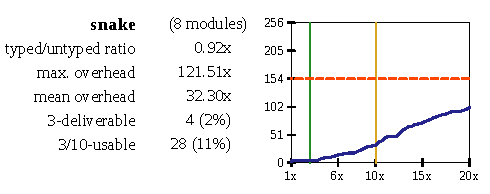
\includegraphics[width=3.5in]{snake} \\
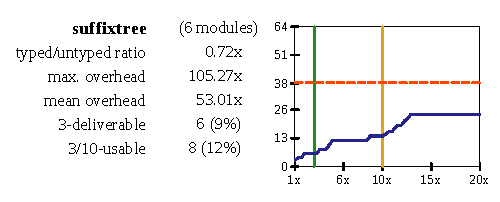
\includegraphics[width=3.5in]{suffixtree}
\end{center}

\footnote{\textit{Is sound gradual typing dead?}
  Takikawa et al. POPL 2016}

}


%===============================================================================
\begin{frame}[fragile]
\frametitle{Casts can cause catastrophic slowdowns}

\begin{center}
\begin{lstlisting}
(define sort!
  : ((Vectorof Dyn) Int Int -> ())
  (lambda ([v : (Vectorof Int)]
       [lo : Int][hi : Int])
    (when (< lo hi)
      (let ([pivot : Int (partition! v lo hi)])
        (sort! v lo (- pivot 1))
        (sort! v (+ pivot 1) hi)))))
\end{lstlisting}
\end{center}

\end{frame}

%===============================================================================
\frame{
\frametitle{Casts can cause catastrophic slowdowns}

\begin{center}
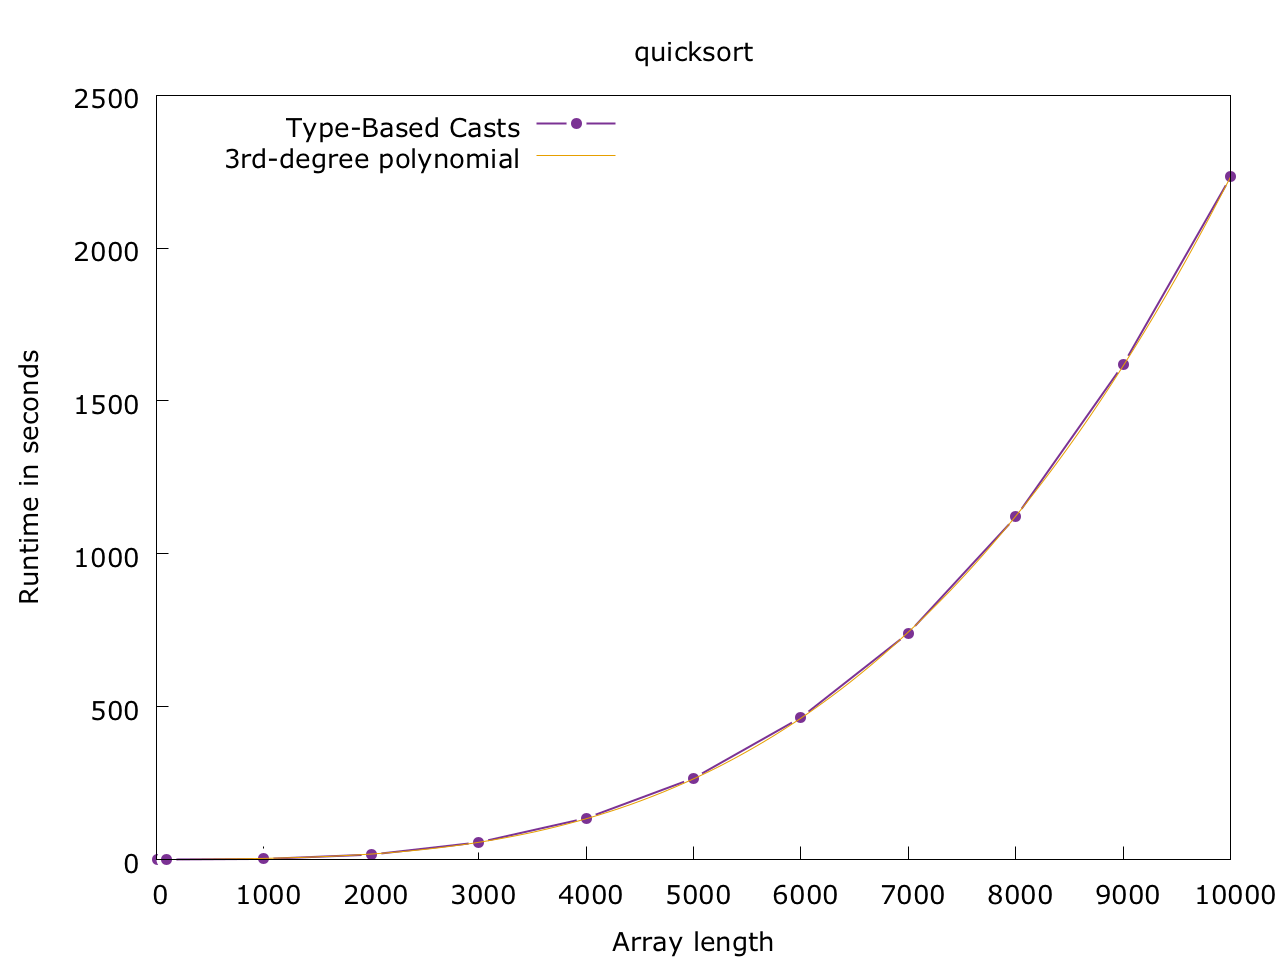
\includegraphics[width=3.5in]{plots/space/quicksort/Type-Based_Casts/poly3fitting.png} \\
\end{center}

}
% ===============================================================================
\frame{
\frametitle{Casts can cause catastrophic slowdowns}

\begin{center}
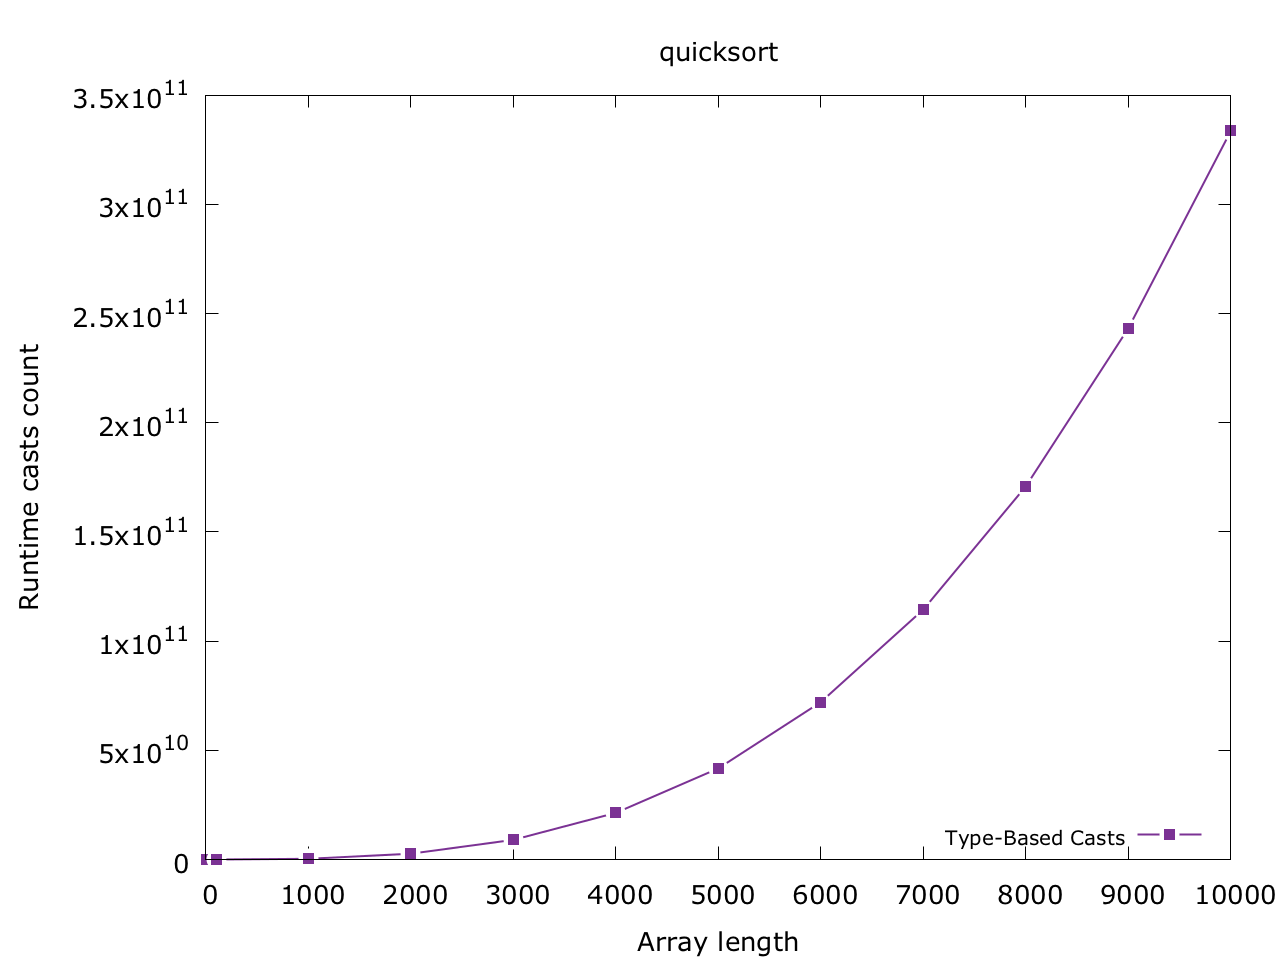
\includegraphics[width=3.5in]{plots/space/quicksort/Type-Based_Casts/casts.png} \\
\end{center}

}
% ===============================================================================
\frame{
\frametitle{Casts can cause long proxy chains}

\begin{center}
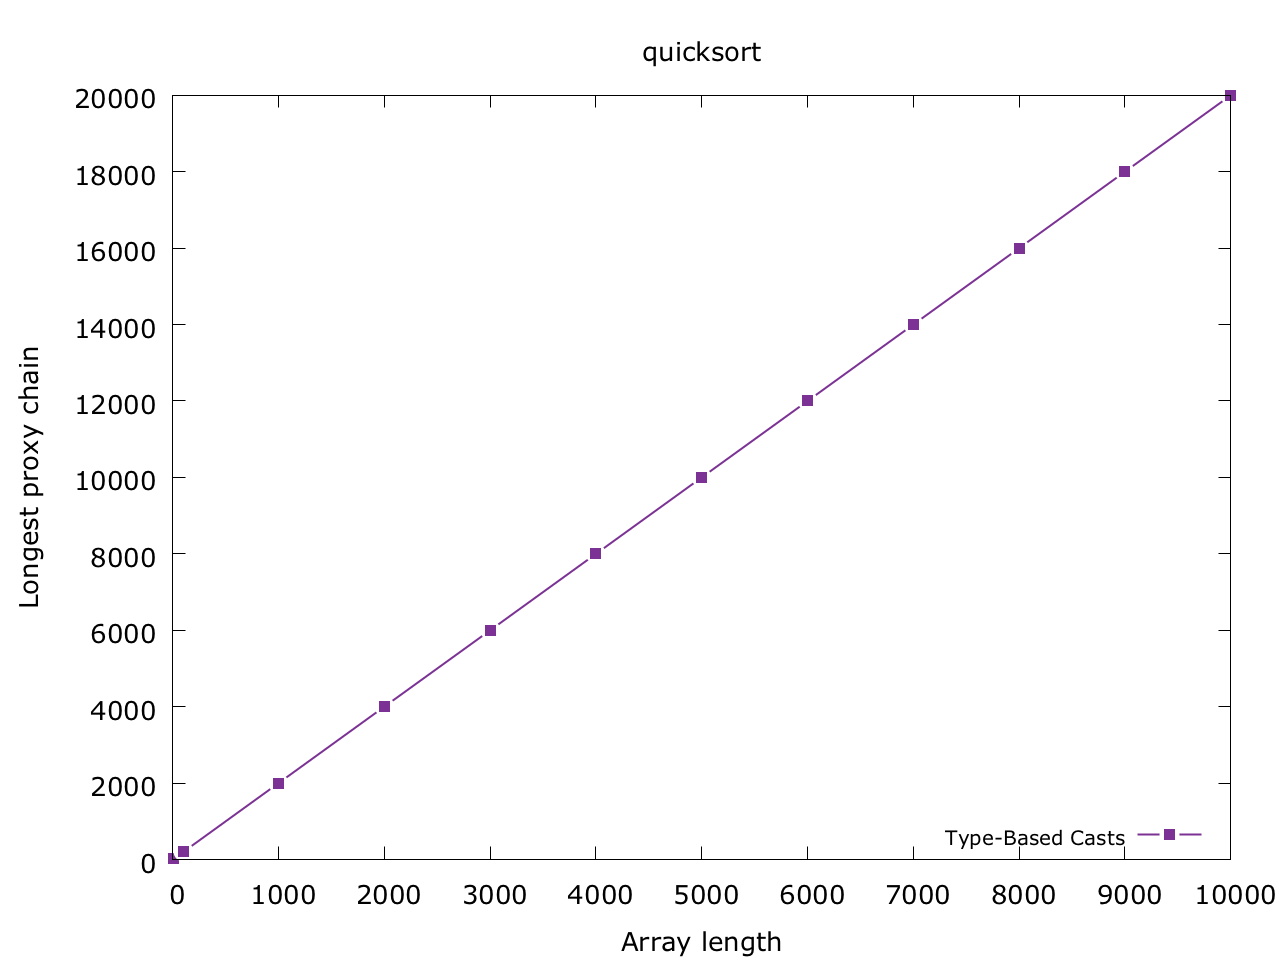
\includegraphics[width=3.5in]{plots/space/quicksort/Type-Based_Casts/lpc.png} \\
\end{center}

}

% ===============================================================================
\frame{
\frametitle{Efficient gradual typing}

\begin{itemize}
\item Challenges to Efficiency
\item \textbf{Challenges to Evaluation}
\item Space-efficient Coercions
\item Monotonic Coercions
\item Performance Comparison
\end{itemize}

}

% ===============================================================================
\frame{
\frametitle{Challenges to Performance Evaluation}

\begin{itemize}
\item Takikawa et al. POPL 2016 proposes to run all the combinations of
  making each module typed or untyped. There are $2^n$
  configurations for a program that consists of $n$ modules.
  \item This should work for most benchmarks where $n$ is relatively
    small.
    \pause
  \item But what if the language supports fine-grained gradual
    typing, where the programmer may opt to not write some type
    annotations or put Dyn inside some?
    \pause
  \item The size of the configuration space for a textbook quicksort is
    248832000000. For n-body, it is
    6914086267191872901144038355222134784.
\end{itemize}

}

%===============================================================================
\frame{
\frametitle{Grift: an experimental compiler}
\begin{itemize}
\item An ahead-of-time optimizing compiler for gradual typing.
\item The source is a functional language with tuples and mutable
  vectors and references, and the target is C.
\item The runtime system implements \textbf{coercions} and
  \textbf{monotonic references}.
\item The compiler specializes casts when their source and/or target
  type is known at compile time.
\item The compiler defers coercion creation until it is actually needed.
\end{itemize}
}

% ===============================================================================

\frame{
\frametitle{Grift Performance Evaluation}

\begin{itemize}
\item a number of configurations are sampled from across the spectrum of
  type precision.
\item Grift is compared on partially typed code to a variant of Grift
  where it is statically typed and does not support gradual typing
  (Static Grift) and to Grift on fully untyped code (Dynamic Grift)
\item Grift is compared on fully typed benchmarks to fully typed
  languages.
\item Grift is compared on fully untyped benchmarks to dynamically typed
  languages.
\end{itemize}

}
% ===============================================================================

\frame{
\frametitle{Efficient gradual typing}

\begin{itemize}
\item Challenges to Efficiency
\item Challenges to Evaluation
\item \textbf{Space-efficient Coercions}
\item Monotonic Coercions
\item Performance Comparison
\end{itemize}

}
% ===============================================================================

\frame{
\frametitle{Compress casts via coercion reduction}

\[
\begin{stack}
\mathit{odd}(0) : \Bool \cast{} \dyn \cast{\ell} \Bool \cast{} \dyn \cast{m} \Bool \cast{} \dyn \\
\\
\mathit{odd}(0) \rd{\CAST{ \pl{\Bool}} \CAST{\qu{\ell}{\Bool}} } \CAST{\pl{\Bool}} \CAST{\qu{m}{\Bool}} \CAST{ \pl{\Bool}}  \\
 \longrightarrow \\
\mathit{odd}(0) \rd{\CAST{\Id{\Bool}} \CAST{ \pl{\Bool}}} \CAST{\qu{m}{\Bool}} \CAST{ \pl{\Bool}}  \\
 \longrightarrow \\
\mathit{odd}(0) \rd{\CAST{ \pl{\Bool}} \CAST{\qu{m}{\Bool}}} \CAST{ \pl{\Bool}}  \\
 \longrightarrow \\
\mathit{odd}(0) \rd{\CAST{\Id{\Bool}} \CAST{ \pl{\Bool}} } \\
 \longrightarrow \\
\mathit{odd}(0) \rd{\CAST{\pl{\Bool}}}
\end{stack}
\]

}
%===============================================================================
\frame{
\frametitle{Coercion Calculus}

%% Blame paths
%% \[
%% p,q ::= \ell \mid p d \mid p r \mid p! \mid p?
%% \]

Syntax
\[
 c,d ::= 
  \Id{T} \mid \pl{I} \mid \qu{\ell}{I} \mid c \to d \mid c \semi d
     \mid \Fail{\ell}
\]
Reduction
\begin{align*}
c ; \Id{T} & \longrightarrow c \\
\Id{T}; c & \longrightarrow c \\
\pl{I} ; \qu{\ell}{I} & \longrightarrow \Id{I}  \\
\pl{I} ; \qu{\ell}{I'} & \longrightarrow \Fail{\ell} & I \neq I' \\
(c \tu d) ; (c' \tu d') & \longrightarrow (c';c) \to (d;d') \\
(\Id{T} \to \Id{T'}) & \longrightarrow \Id{T \to T'} \\
\Fail{\ell}; c & \longrightarrow \Fail{\ell} \\
c;\Fail{\ell} & \longrightarrow \Fail{\ell} &
 \text{if } c \neq \qu{\ell'}{I}
\end{align*}


\footnote{\textit{Dynamic Typing.} Henglein. ESOP 1992}
%\footnote{\textit{Blame and coercion.} Siek, Thiemann, Wadler. PLDI 2015.}
}

%===============================================================================
\frame{
\frametitle{Normalize adjacent coercions}

\begin{align*}
  e &::= \cdots \mid e \CAST{c} & \text{Terms}\\
  u & ::= n \mid \lam{x \of T}e
  & \text{Uncoerced Values} \\
  v & ::=
   u \mid u \CAST{c \tu d} \mid u \CAST{ \pl{I} } 
  & \text{Values}
  %% \EE & ::=  
  %%  \FF \mid \FF[\Hole \CAST{c}] 
  %% & \text{Evaluation contexts}\\
  %% \FF & ::= 
  %%  \Hole \mid \EE[\Hole \app e] \mid \EE[v \app \Hole]
  %% &\text{Cast-free contexts}
\end{align*}
\begin{align*}
  (u \CAST{c \tu d}) \app v
    & \reduce (u \app v \CAST{c}) \CAST{d} \\
    % \label{WrapT}\tagsc{Wrap} \\
  u \CAST{\Id{T}}
    & \reduce u \\
  \rd{e \CAST{c} \CAST{d}}
    & \rd{\reduce e \CAST{c'}} & \text{if } (c;d) \longrightarrow^{*}c'\\
    % \label{ComposeT}\tagsc{Compose} \\
  u \CAST{\bot^\ell}
    & \reduce \blame{\ell}  
\end{align*}
\footnote{\textit{Space-Efficient Gradual Typing.}
  Herman, Tomb, Flanagan. TFP 2006.}
}

%===============================================================================
\frame{
\frametitle{Coercions in normal form \& composition}
\small

\[
\begin{stack}
  % \text{Threesome coercions}
  s,t ::=
   \Id{\dyn} \mid (\qu{\ell}{I} \semi i) \mid i \\
  % \text{Injection coercions}
  i ::= 
   (g \semi \pl{I}) \mid g \mid \FAIL{I}{\ell}{H} \qquad\qquad
  % \text{Ground coercions}
  g,h ::= 
   \Id{\Int} \mid (s \to t) 
\end{stack}
\]
 \hfill \fbox{$s \fatsemi t = s$}
\vspace{-10pt}
\begin{align*}
  \Id{\Int} \fatsemi t = \Id{\dyn} \fatsemi t & = t \\
  (s \to t) \fatsemi (s' \to t') & = (s' \fatsemi s) \to (t \fatsemi t') \span \\
  (g \semi \pl{I}) \fatsemi \Id{\dyn} & = g \semi \pl{I} \\
  (\qu{\ell}{I} \semi i) \fatsemi t & = \qu{\ell}{I} \semi (i \fatsemi t)  \\
  g \fatsemi (h \semi \pl{I}) & = (g \fatsemi h) \semi \pl{I}  \\
  (g \semi \pl{I}) \fatsemi (\qu{\ell}{I} \semi i) & = g \fatsemi i \\
  (g \semi \pl{I}) \fatsemi (\qu{\ell}{I'} \semi i) & = \FAIL{I}{\ell}{I'}
    & \text{if $I \neq I'$} \\
  \FAIL{I}{\ell}{I'} \fatsemi s  = 
  g \fatsemi \FAIL{I}{\ell}{I'} & = \FAIL{I}{\ell}{I'}
\end{align*}
\[
 \FF[e \CAST{s} \CAST{t}]
    \reduce \FF[e \CAST{s \fatsemi t}]
\]
\footnote{\textit{Blame and coercion $\ldots$} Siek, Thiemann, Wadler. PLDI 2015.}
}
%===============================================================================
\frame{
\frametitle{Coercions eliminate catastrophic slowdowns}

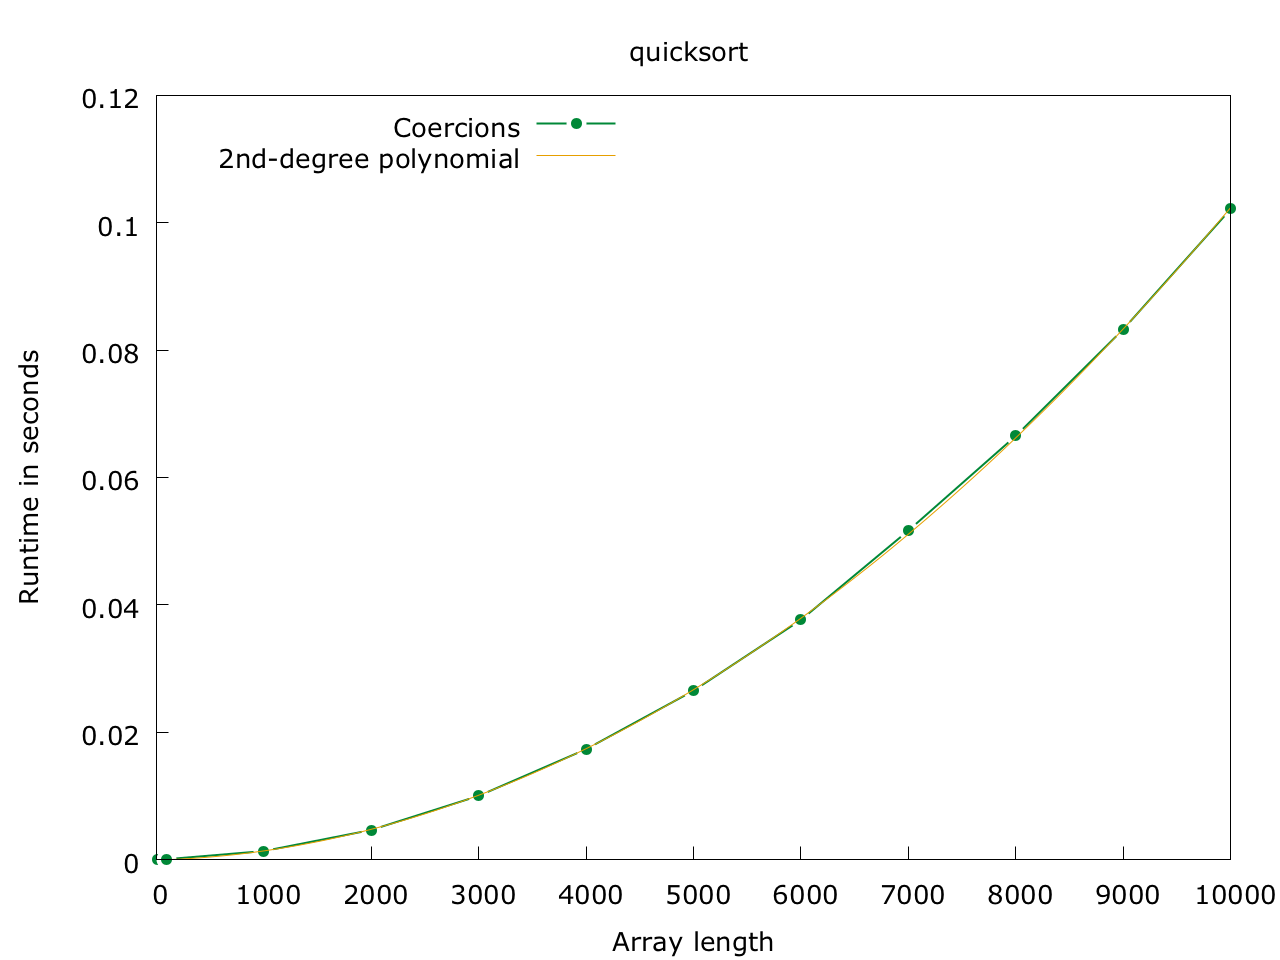
\includegraphics[width=4in]{plots/space/quicksort/Coercions/poly2fitting.png}

}
% ===============================================================================
\frame{
\frametitle{Coercions eliminate catastrophic slowdowns}

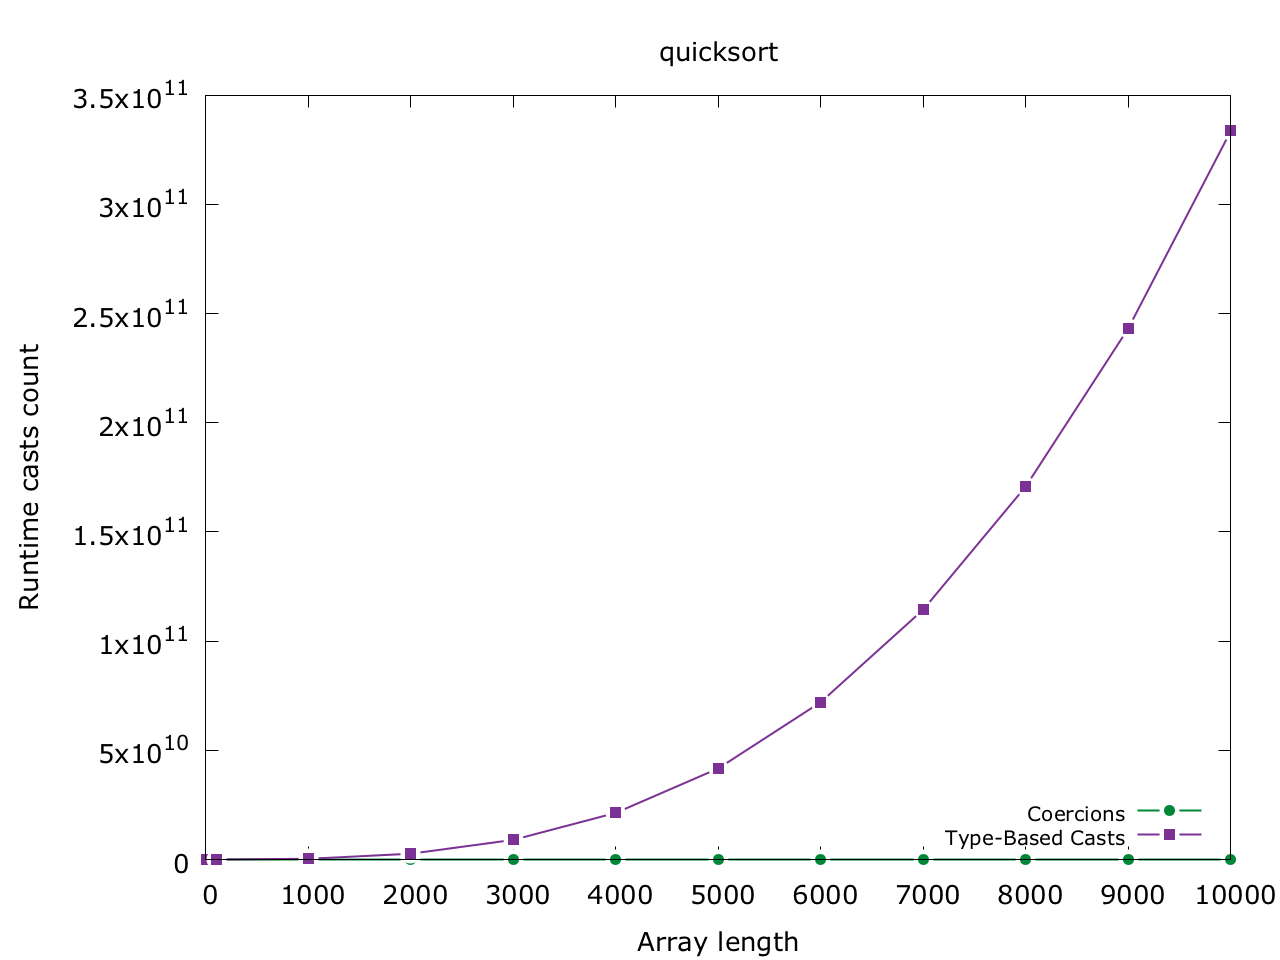
\includegraphics[width=4in]{plots/space/quicksort/casts.png}

}
% ===============================================================================
\frame{
\frametitle{Coercions eliminate catastrophic slowdowns}

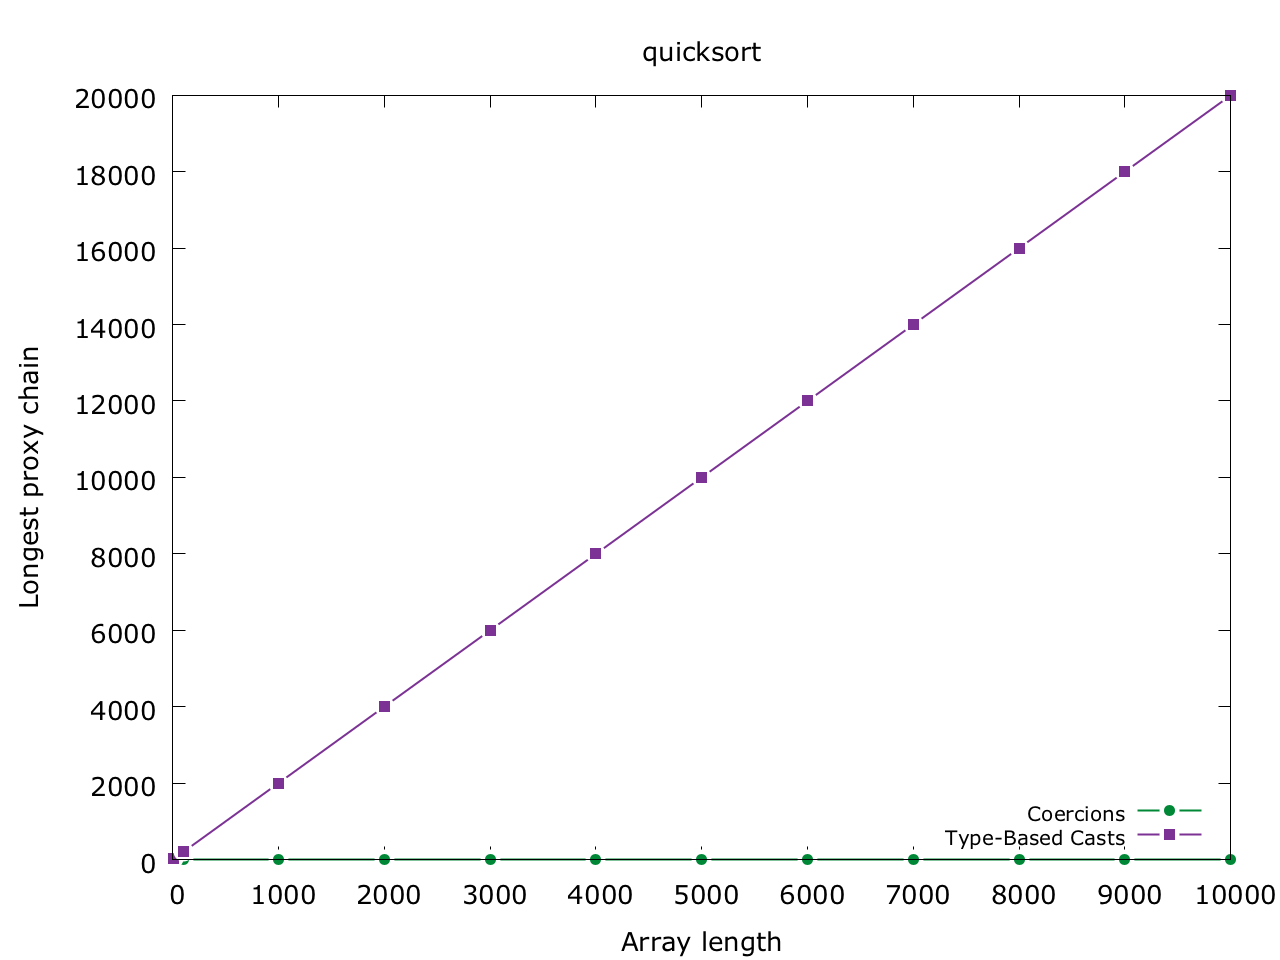
\includegraphics[width=4in]{plots/space/quicksort/lpc.png}

}
% ===============================================================================
\frame{
\frametitle{Coercions eliminate catastrophic slowdowns}

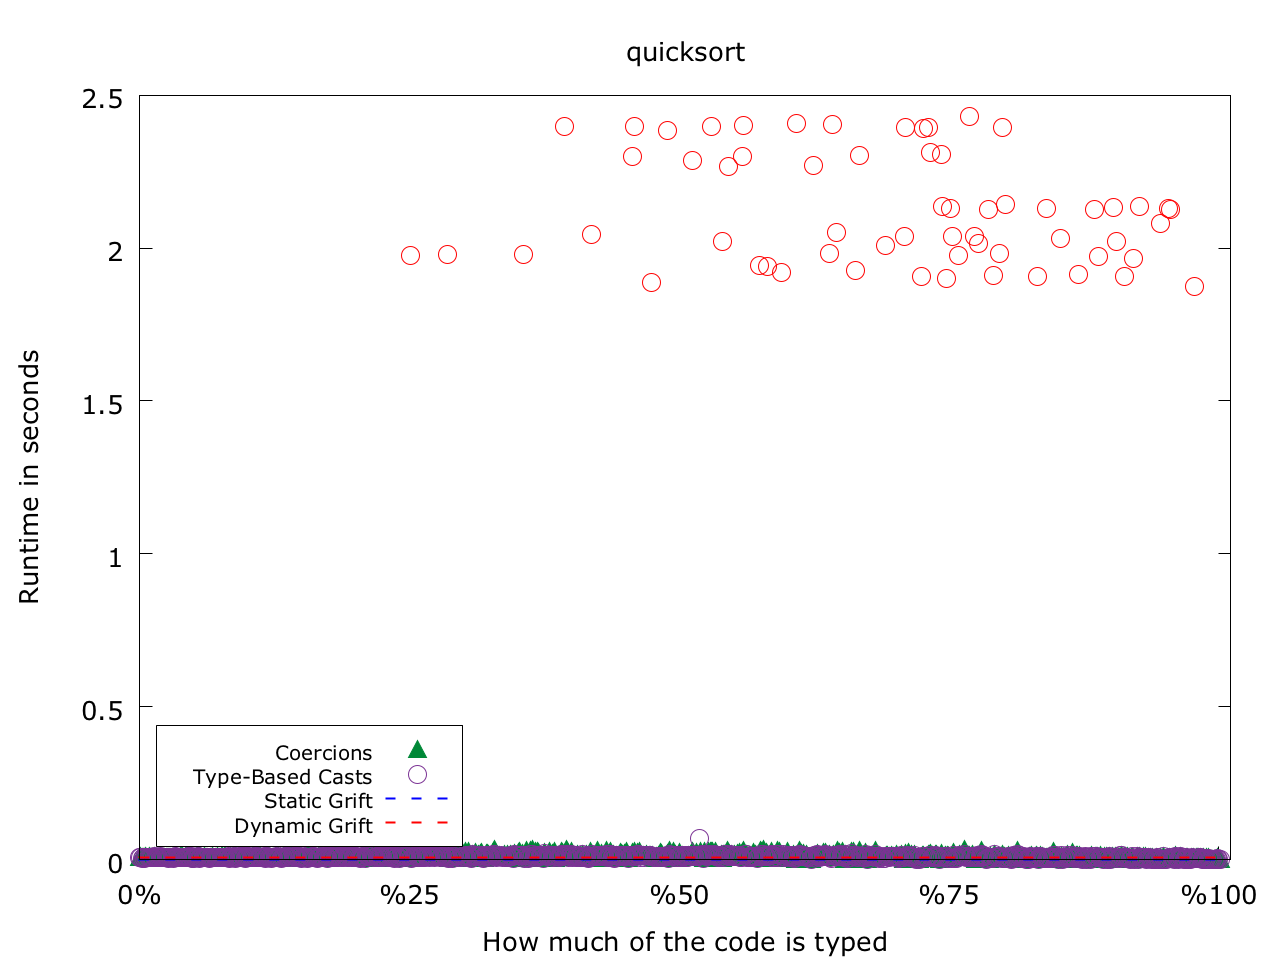
\includegraphics[width=4in]{plots/casts-or-coercions/quicksort/rt.png}
\begin{itemize}
  \item mean speedup of $\kw{13}$ and max speedup of $\kw{1756}$
\end{itemize}
}
%===============================================================================
\frame{
\frametitle{Coercions sometimes incur overhead}

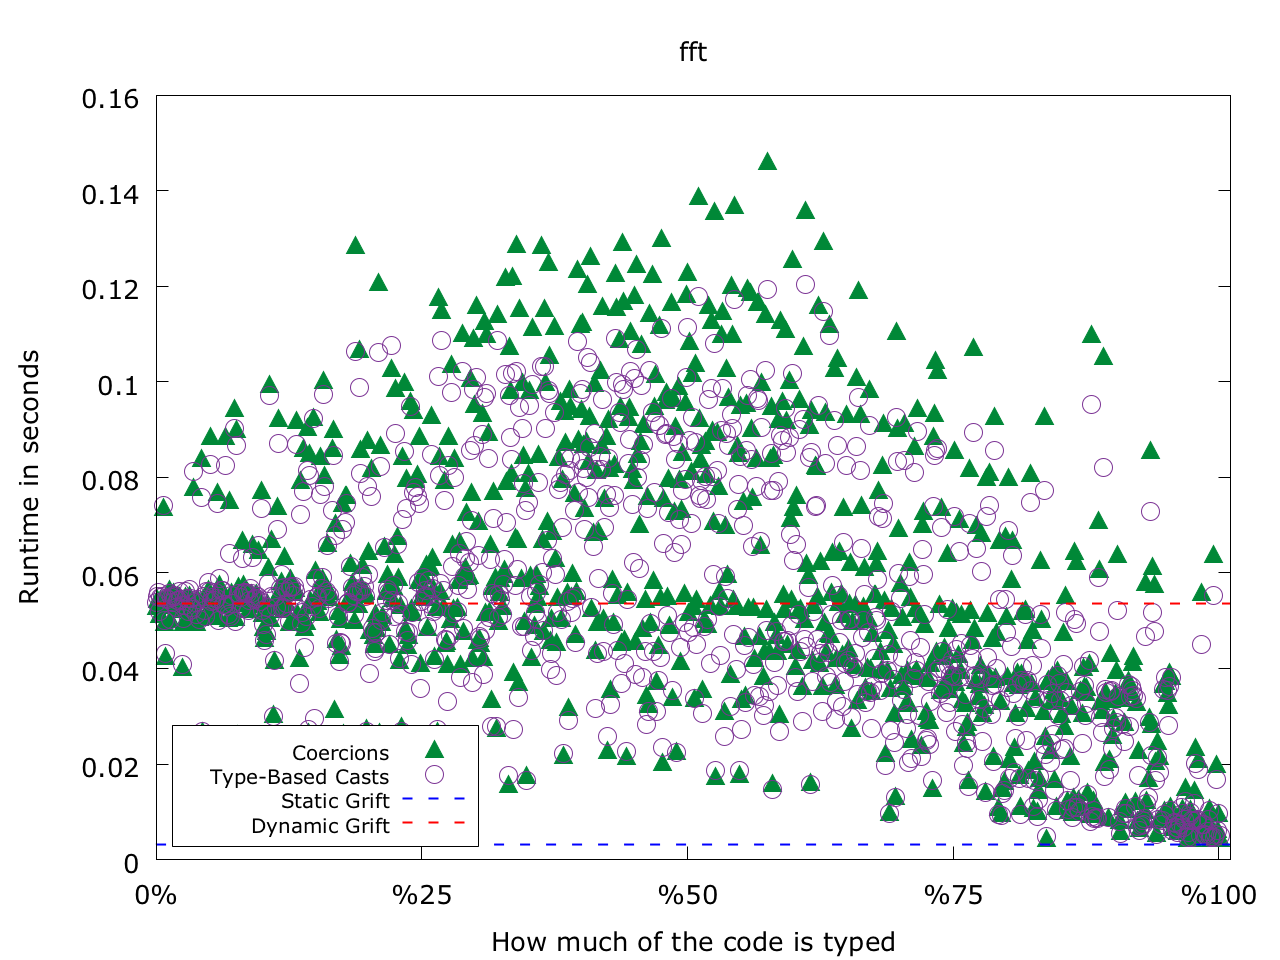
\includegraphics[width=4in]{plots/casts-or-coercions/fft/rt.png}
\begin{itemize}
  \item mean slowdown of $\kw{1.1}$ and max slowdown of $\kw{1.6}$
\end{itemize}

}
%===============================================================================
\frame{
\frametitle{Coercions sometimes pay for themselves}

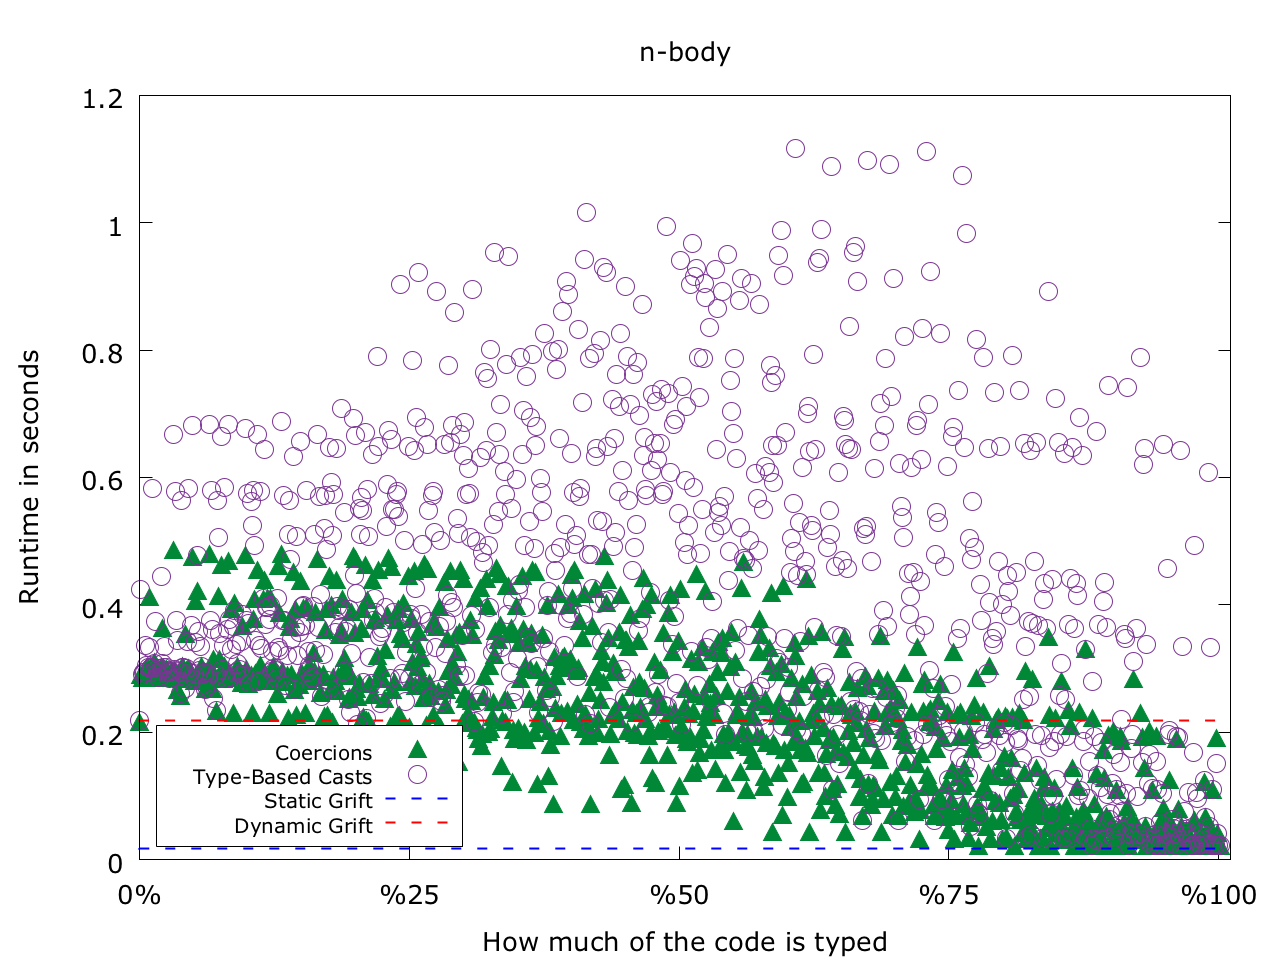
\includegraphics[width=4in]{plots/casts-or-coercions/n_body/rt.png}
\begin{itemize}
  \item mean speedup of $\kw{1.9}$ and max speedup of $\kw{28}$
\end{itemize}

}
% ===============================================================================

\frame{
\frametitle{Coercions sometimes pay for themselves}

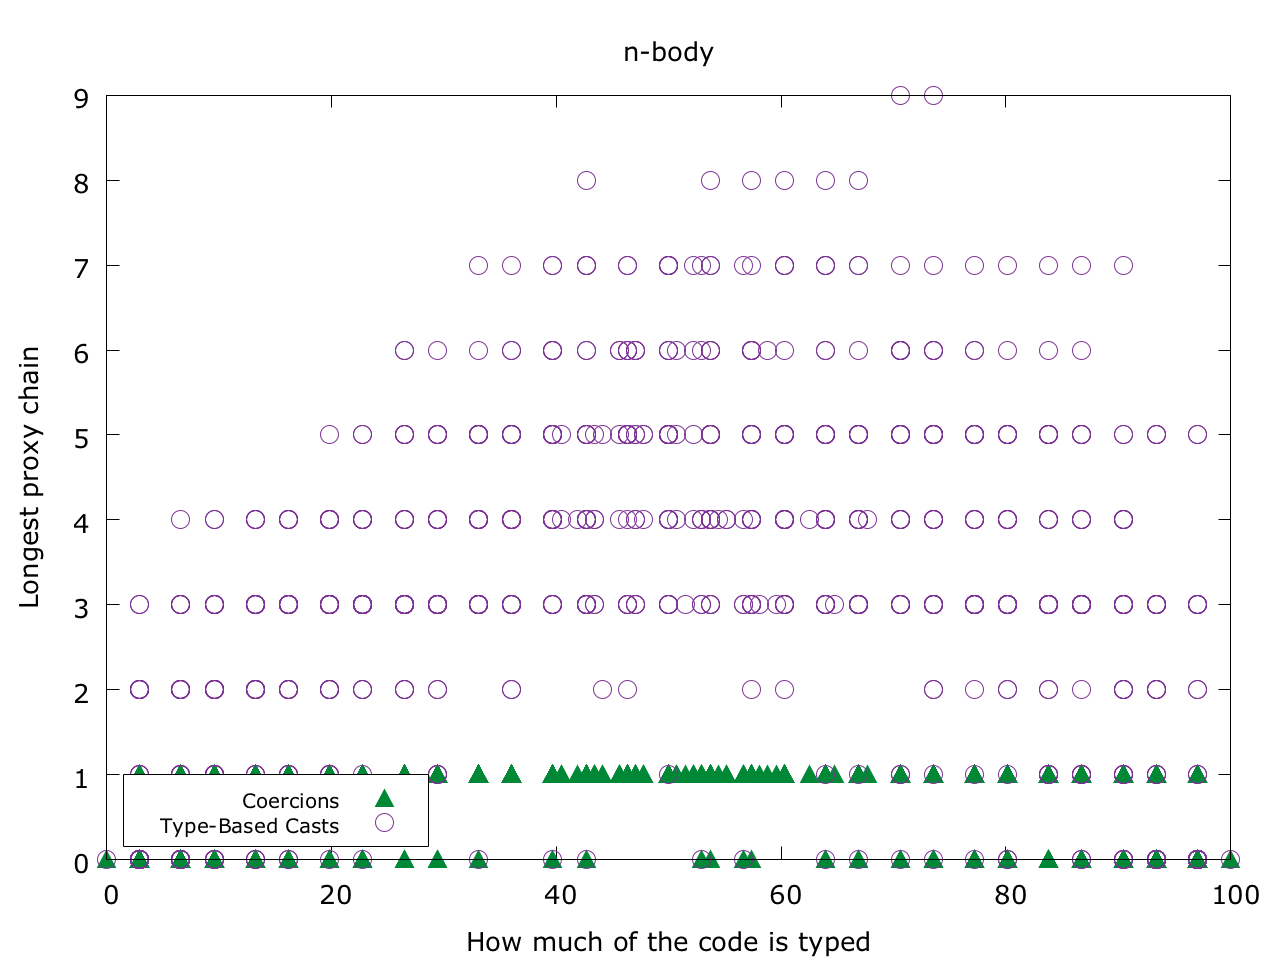
\includegraphics[width=4in]{plots/casts-or-coercions/n_body/lpc.png}

}
%===============================================================================
\frame{
\frametitle{Efficient gradual typing}

\begin{itemize}
\item Challenges to Efficiency
\item Challenges to Evaluation
\item Space-efficient Coercions
\item \textbf{Monotonic Coercions}
\item Performance Comparison
\end{itemize}

}
%===============================================================================
\frame{
\frametitle{Gradual typing with mutable references}
\vspace{5pt}
\begin{align*}
  T & ::= \cdots \mid \Ref T \\
  e & ::= \cdots \mid \alloc e \mid \deref^\ell e \mid e \update^\ell e \\
  v & ::= \cdots \mid a \mid a \CAST{\Ref (c,d)}
\end{align*}
Consistency \hfill \fbox{$T \sim T$}
\[
\cdots
\qquad
\inference
  {T_1 \sim T_2}
  {\Ref T_1 \sim \Ref T_2}
\]

Coercions
\[
c ::= \ldots \mid \Ref(c_1, c_2)
\]

Compile Casts to Coercions
\begin{align*}
  \bcfun{\Ref T_1 \cast{\ell} \Ref T_2}
    &=  \Ref(\bcfun{T_1 \cast{\ell} T_2}, \bcfun{T_2 \cast{\ell} T_1})
\end{align*}

\footnote{\textit{Space-Efficient Gradual Typing.}
  Herman, Tomb, Flanagan. TFP 2006.}

}
%===============================================================================
\frame[containsverbatim]{
\frametitle{Example of overhead in reference access}

\begin{minipage}{0.6\textwidth}
\begin{lstlisting}
fun f(p3:Ref Int, p4:Ref Int)=
    !p3 + !p4;
\end{lstlisting}
\hrule
\begin{lstlisting}
val p1 = ref 5;
val p2 = ref (6|<Int!>|);

f(p1, p2|<Ref(Int?,Int!)>|);


|ref(Int?,Int!)| 
  : Ref $\dyn$ $\Rightarrow$ Ref Int
\end{lstlisting}
\end{minipage}
\vrule
\begin{minipage}{0.38\textwidth}
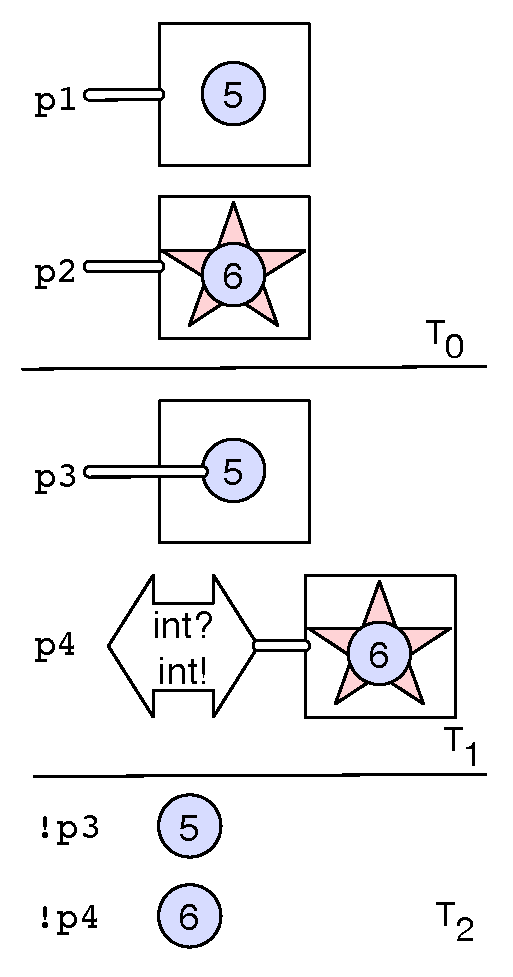
\includegraphics[height=2.65in]{HermanRefCoerce}
\end{minipage}

\fbox{
\begin{minipage}{\textwidth}
Problem: generated code for \lstinline{!p3} and \lstinline{!p4}
must branch at runtime for the two kinds of references.
\end{minipage}
}

}
%===============================================================================
\frame{
\frametitle{Root of the problem}

\begin{theorem}[Canonical Forms]
Suppose $\emptyset \vdash v : T$. If $T=\Ref T$, then either
\begin{itemize}
\item $v = a\;$ for some address $a$, or
\item $v = a \CAST{\Ref(c_1, c_2)}$.
\end{itemize}
\end{theorem}

Two rules for dereference
\begin{align*}
\deref a, \mu & \reduce \mu(a), \mu  \\
\deref (a\CAST{\Ref(c_1, c_2)}),\mu & 
    \reduce (\deref a)\CAST{c_1} , \mu\\
\end{align*}
Two rules for update
\begin{align*}
a \update v, \mu & \reduce a, \mu(a \mapsto v) \\
a \CAST{\Ref(c_1,c_2)} \update v, \mu  & 
    \reduce a \update v \CAST{c_2} , \mu
\end{align*}

}
%===============================================================================
\frame[containsverbatim]{
\frametitle{Monotonic References}

\begin{minipage}{0.6\textwidth}
\begin{lstlisting}
fun f(p3:Ref Int, p4:Ref Int)=
    !p3 + !p4;
\end{lstlisting}
\hrule
\begin{lstlisting}
val p1 = ref 5;
val p2 = ref (6|<Int!>|);

f(p1, p2|<Ref(Int)>|);



$ $
\end{lstlisting}
\end{minipage}
\vrule
\begin{minipage}{0.38\textwidth}
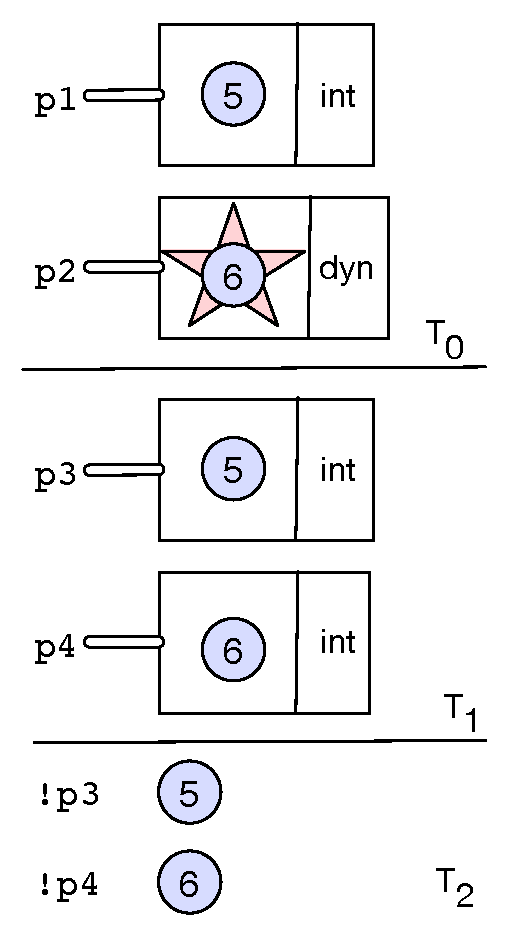
\includegraphics[height=2.6in]{MonoRefCoerce}
\end{minipage}
\fbox{
\begin{minipage}{\textwidth}
Update the reference cell to the \emph{meet} of the
current RTTI and the target of the cast.
\end{minipage}
}

\footnote{\textit{Monotonic Ref. for Efficient Gradual Typing.}
  Siek et al. ESOP 2015}

}
%===============================================================================

\frame[containsverbatim]{
\frametitle{Aliasing and Static vs. Dynamic Dereference}

\vspace{10pt}

\begin{minipage}{0.6\textwidth}
\begin{lstlisting}
fun f(x:Ref Int, y:Ref $\dyn$)=
    ~!x~ + |!y@$\rd{\dyn}$|;

p = ref (2|<Int!>|);
f(p, p);
\end{lstlisting}
\end{minipage}
\vrule
\quad
\begin{minipage}{0.35\textwidth}
Compile-time choice:
\begin{itemize}
\item {\color{blue} Fast static deref.}
\item {\color{red} Slow dynamic dereference}
\end{itemize}
\end{minipage}

\begin{center}
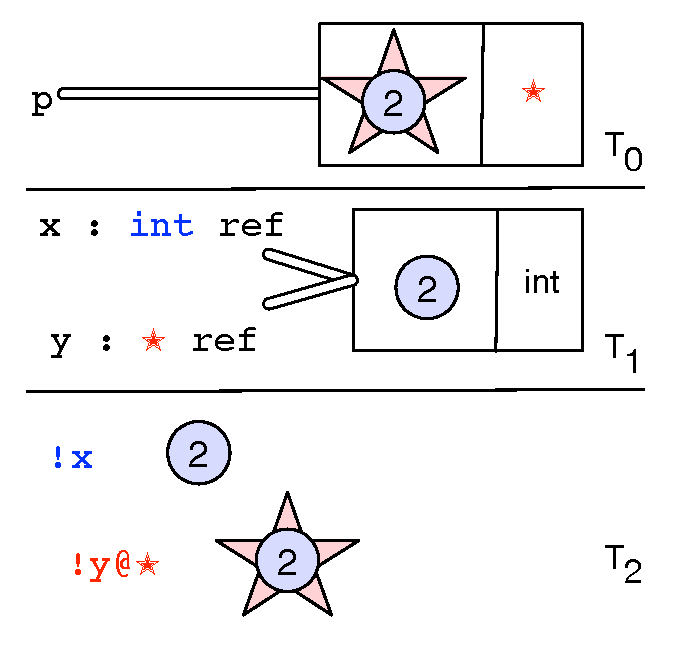
\includegraphics[height=2in]{MonoAlias}
\end{center}
}


%===============================================================================

\frame{
\frametitle{The Monotonic Invariant}

\begin{minipage}{0.8\textwidth}
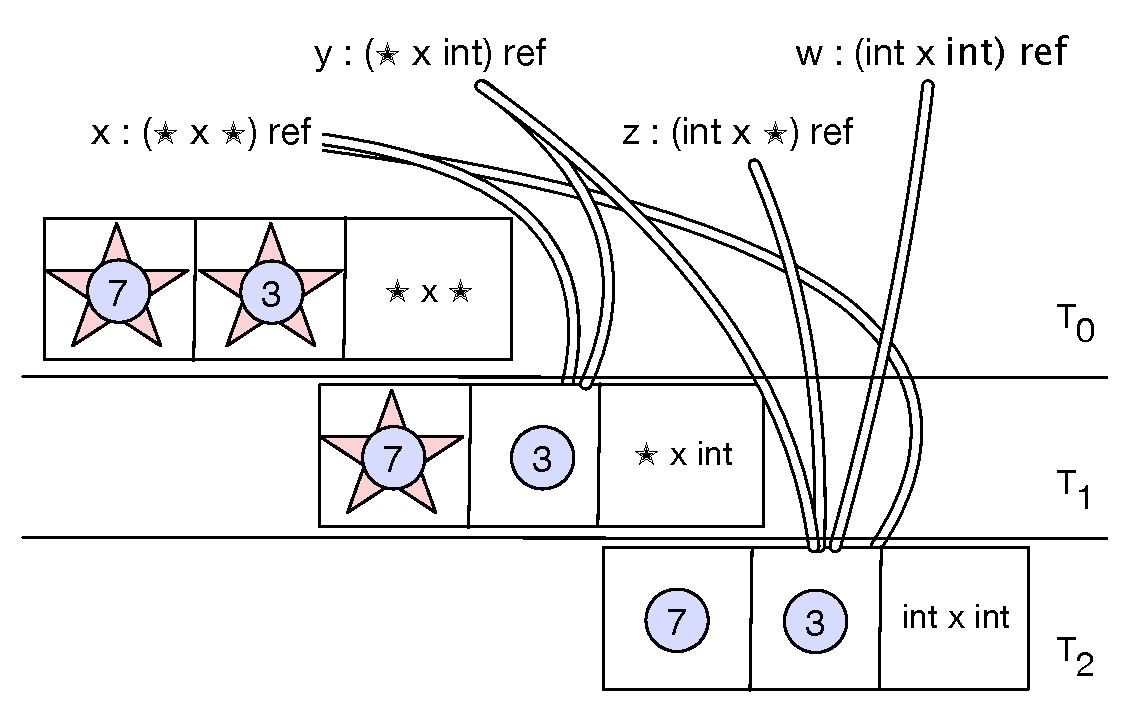
\includegraphics[height=2in]{MonoInvariant}
\end{minipage}
\begin{minipage}{0.2\textwidth}
\xymatrix{
  \Dyn \times \Dyn  \ar[d]^{\sqsubseteq}\\
  \Dyn \times \Int \ar[d]^{\sqsubseteq} \\
  \Int \times \Int
}
\end{minipage}

\fbox{
\begin{minipage}{\textwidth}
\begin{itemize}
\item The RTTI of a cell may become more precise. 
\item Every reference is less or equally precise as the RTTI. 
\item If a reference is fully static (e.g. w), then so is the cell.
\end{itemize}
\end{minipage}
}

}
%===============================================================================
\frame{
\frametitle{Monotonic implementation}

\begin{itemize}
\item hashconsing types at runtime to speedup the meet operation
\item casted tuple values are just copies of the original tuples written
  to the heap and updated in place while the cast is in progress.
\end{itemize}

}
%===============================================================================
\frame{
\frametitle{Monotonic eliminates overhead in static code}

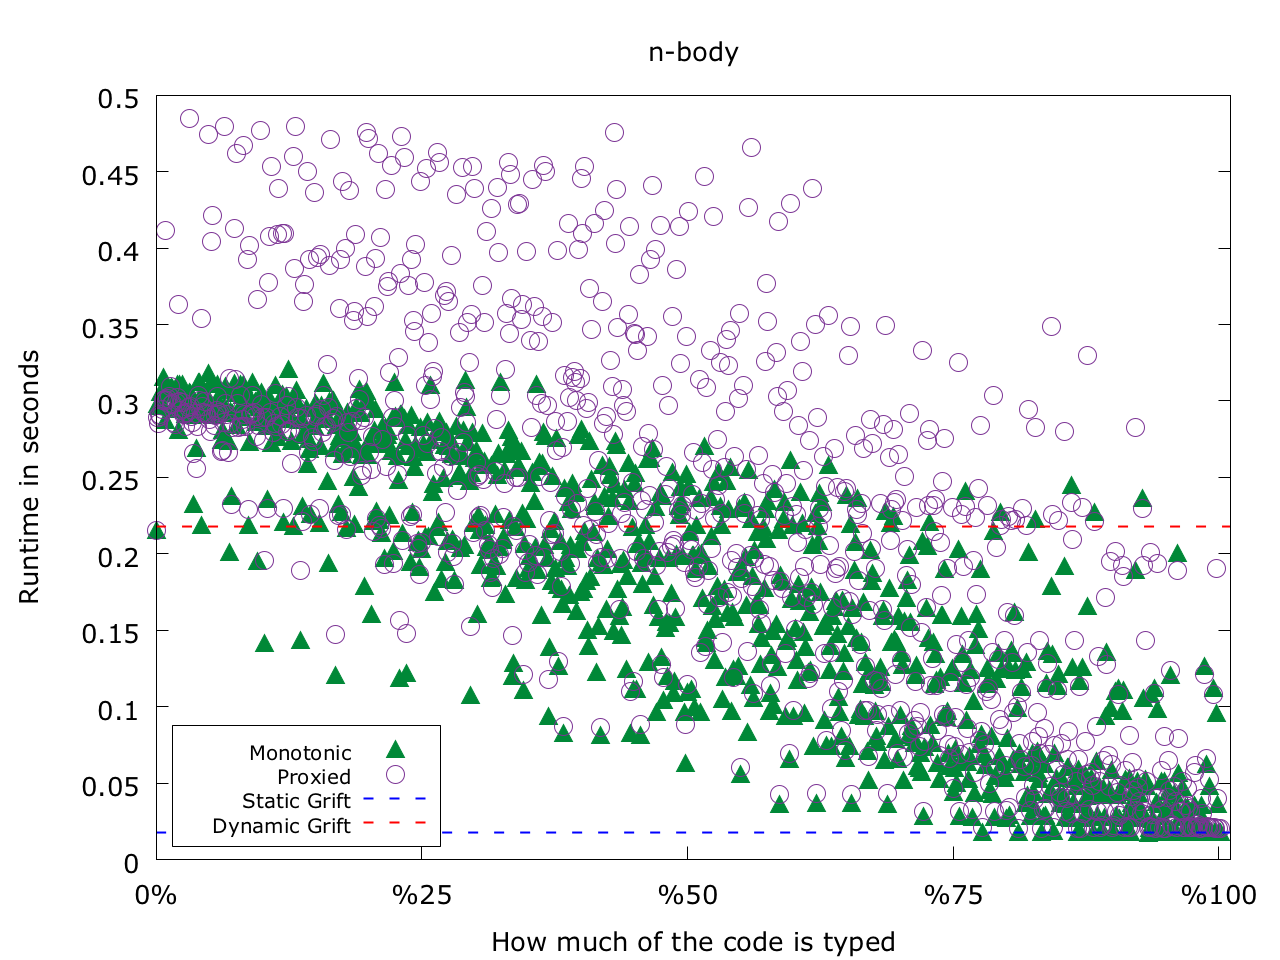
\includegraphics[width=4in]{plots/monotonic-v-coercions/n_body/rt.png}

\begin{itemize}
  \item mean speedup of 1.26 and max speedup of 3.24
\end{itemize}

}
%===============================================================================
\frame{
\frametitle{Montonic doesn't matter for some programs}

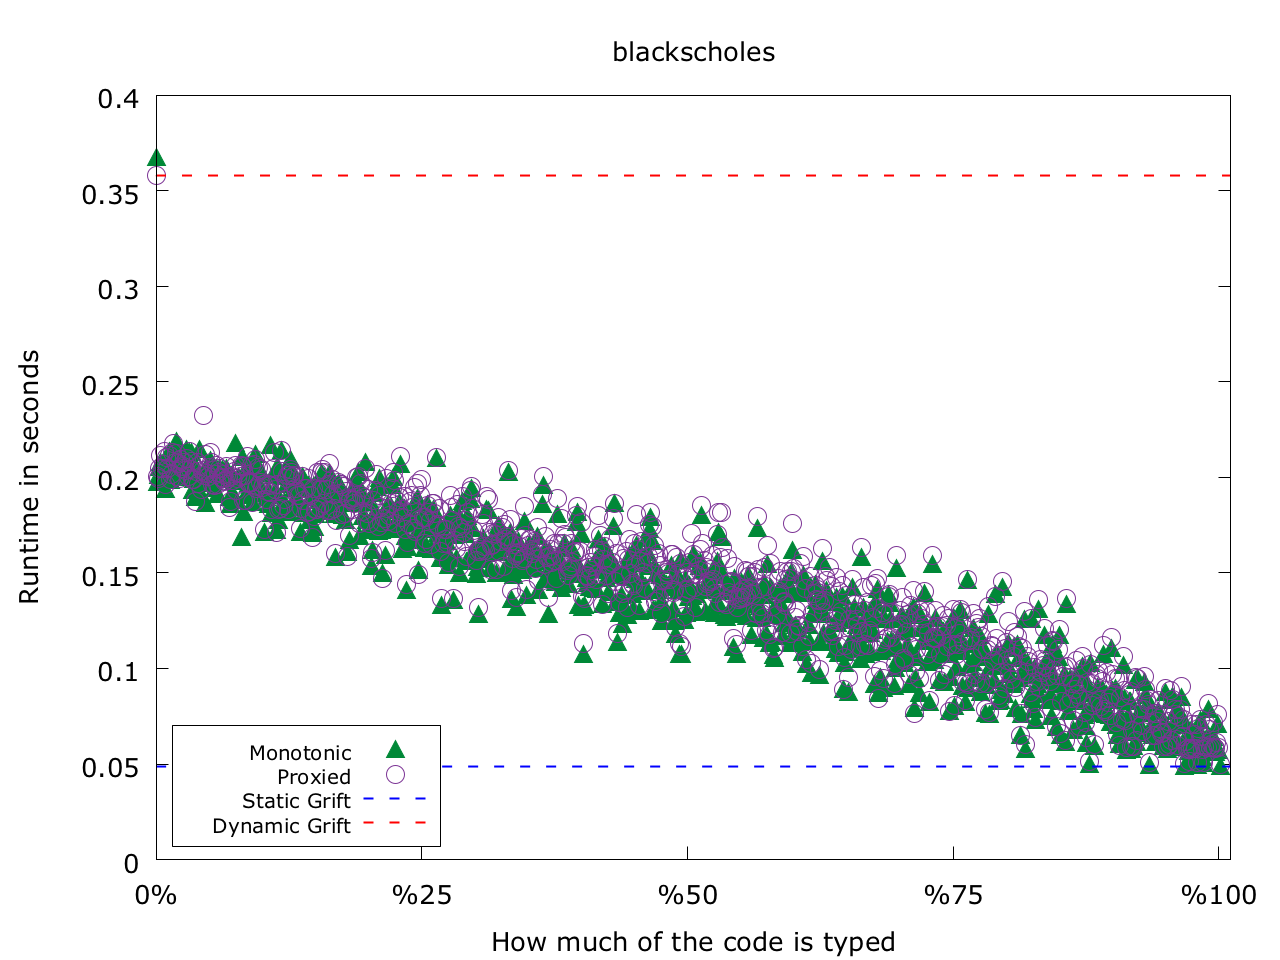
\includegraphics[width=4in]{plots/monotonic-v-coercions/blackscholes/rt.png}

}
%===============================================================================
\frame{
\frametitle{Efficient gradual typing}

\begin{itemize}
\item Challenges to Efficiency
\item Challenges to Evaluation
\item Space-efficient Coercions
\item Monotonic Coercions
\item \textbf{Performance Comparison}
\end{itemize}

}
%===============================================================================


%% to do: specialization

%===============================================================================
\frame{
\frametitle{Comparison on dynamically typed programs}

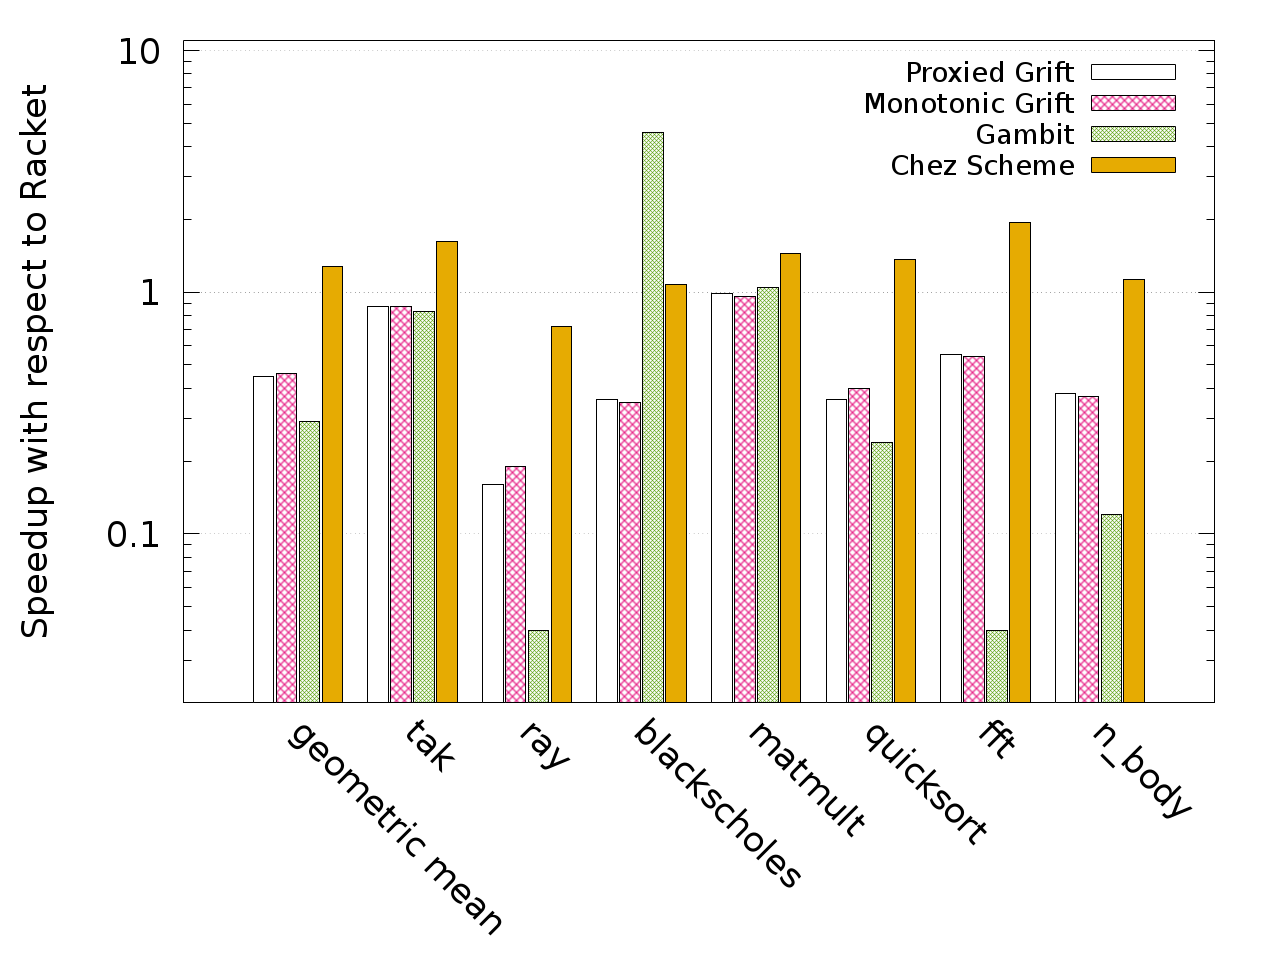
\includegraphics[width=4in]{plots/external/Specialized_Lazy_Coercions_dynamic.png}

}
%===============================================================================
\frame{
\frametitle{Comparison on statically typed programs}

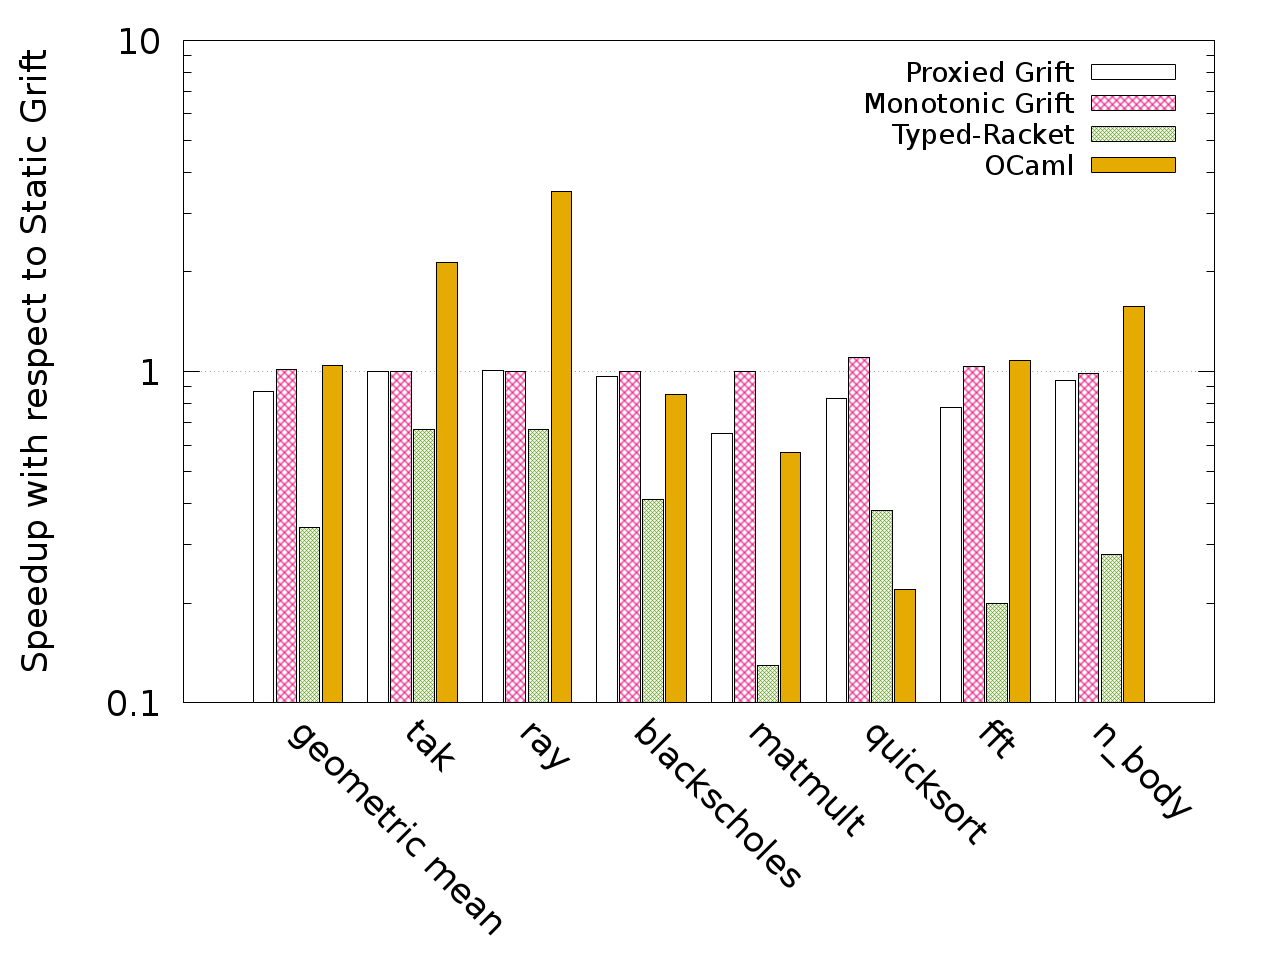
\includegraphics[width=4in]{plots/external/Specialized_Lazy_Coercions_static.png}

}
%===============================================================================
\frame{
\frametitle{Conclusion}

\begin{itemize}
\item Gradual typing can be efficient!
\item On dynamically typed code: competative with Gambit.
\item On statically typed code: competative with OCaml.
\item On partially typed code, performance varies roughly between \%50
  of untyped impl. to \%100 of typed impl.
\item Use \textbf{coercions} to eliminate catastrophic slowdowns
  in partially typed code.
\item Use \textbf{monotonic references} to reduce overhead in
  statically typed code.
\end{itemize}


}

%===============================================================================
\frame{
\frametitle{}

\center{Grift is open source: github.com/Gradual-Typing/Grift}
\vspace{0.7in}
\center{\Large Thank you!}


}

\end{document}

% LocalWords:  titlepage containsverbatim frametitle  Siek Taha lstlisting
% LocalWords:  Rightarrow
% LocalWords:  texttt Rightarrow texttt texttt Rightarrow Findler deriv Wadler
% LocalWords:  Longrightarrow Longrightarrow circ Wrigstad ldots inc bytecode
% LocalWords:  includegraphics invokedynamic switchpoints unboxed xymatrix rrr
% LocalWords:  vspace newsavebox DistExample lrbox linewidth mathtt mathtt emph
% LocalWords:  vdash usebox mathbf mathit longmapsto mathsf subtyping emptyset
% LocalWords:  Henglein's footnotesize Drossopoulou Igarashi Gronski Dimoulas
% LocalWords:  varphi eval Jython microbenchmarks Fibonnaci vitousek bharadwaj
% LocalWords:  Shashank 
